\begin{tabular}{ c c c }
\adjustbox{valign=m}{%
\begin{lstlisting}[language=C++, basicstyle=\ttfamily\small]
if (x > 0) y = 10;
else       y = 20;
\end{lstlisting}
}
&
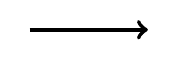
\begin{tikzpicture}
    \draw[->, line width=1.5pt] (0,0) -- (1.5,0);
\end{tikzpicture}
&
\adjustbox{valign=m}{%
\begin{lstlisting}[language=C++, basicstyle=\ttfamily\small]
y = (x > 0)  * 10 + 
    (x <= 0) * 20;
\end{lstlisting}
}
\end{tabular}